
\documentclass[review]{elsarticle}

\usepackage{lineno}

\usepackage{amsmath}
\usepackage{amsfonts}
\usepackage{amsthm}
%\usepackage{url}
\usepackage{subfig}
\DeclareMathOperator*{\argmin}{argmin}
\newcommand*{\argminl}{\argmin\limits}
\newtheorem{prop}{Proposition}
\newtheorem{corollary}{Corollary}

\modulolinenumbers[5]

\journal{Statistics and Probability Letters}

%%%%%%%%%%%%%%%%%%%%%%%
%% Elsevier bibliography styles
%%%%%%%%%%%%%%%%%%%%%%%
%% To change the style, put a % in front of the second line of the current style and
%% remove the % from the second line of the style you would like to use.
%%%%%%%%%%%%%%%%%%%%%%%

%% Numbered
%\bibliographystyle{model1-num-names}

%% Numbered without titles
%\bibliographystyle{model1a-num-names}

%% Harvard
%\bibliographystyle{model2-names.bst}\biboptions{authoryear}

%% Vancouver numbered
%\usepackage{numcompress}\bibliographystyle{model3-num-names}

%% Vancouver name/year
%\usepackage{numcompress}\bibliographystyle{model4-names}\biboptions{authoryear}

%% APA style
%\bibliographystyle{model5-names}\biboptions{authoryear}

%% AMA style
%\usepackage{numcompress}\bibliographystyle{model6-num-names}

%% `Elsevier LaTeX' style
\bibliographystyle{elsarticle-num}
%%%%%%%%%%%%%%%%%%%%%%%

\begin{document}

\begin{frontmatter}

\title{A Stopped Negative Binomial Distribution}
\tnotetext[mytitlenote]{This research was supported by grants R01CA131301, 
R01CA157749, R01CA148996, R01CA168733, and PC50CA196530 awarded by the 
National Cancer Institute along with support from the Yale Comprehensive Cancer 
Center and the Yale Center for Outcomes Research. We would also like 
to thank Rick Landin at Ignyta Inc. for his suggestions.}

%% Group authors per affiliation:
%\author{Elsevier\fnref{myfootnote}}
%\address{Radarweg 29, Amsterdam}
%\fntext[myfootnote]{Since 1880.}

%% or include affiliations in footnotes:
\author[mymainaddress]{Michelle DeVeaux}
\ead{michelle.deveaux@yale.edu}

\author[mymainaddress]{Michael J. Kane\corref{mycorrespondingauthor}}
\cortext[mycorrespondingauthor]{Corresponding author}
\ead{michael.kane@yale.edu}

\author[mymainaddress]{Daniel Zelterman}
\ead{daniel.zelterman@yale.edu}

\address[mymainaddress]{Department of Biostatistics\\ School of Epidemiology and Public Health\\ Yale University, New Haven, CT}

\begin{abstract}
We introduce a discrete distribution suggested by curtailed
sampling rules common in early-stage clinical trials. We derive the
distribution of the smallest number of independent and identically
distributed Bernoulli trials needed to observe either $s$ successes 
or $t$ failures. This report provides a closed-form expression for the 
mass function and illustrates limiting approximations.
\end{abstract}

\begin{keyword}
discrete distribution\sep curtailed sampling
\end{keyword}

\end{frontmatter}

\linenumbers

\section{Introdution and Motivation}

Consider a prototypical early phase, single-arm clinical trial in which 
12 patients
are enrolled and treated. The binomial probability of success is $p=0.045$ for
each patient under the null hypothesis that treatment is not effective.
If two or more patients out of these 12 respond to the treatment then we 
reject this null
hypothesis and the treatment is deemed successful at significance 
level of $0.1$.  If fewer than two respond then the null is not rejected
and the treatment is judged as ineffective.

If all 12 patients are enrolled at once, as in the classic
design, then the sample size is 12. However, in most clinical trials the
patients are enrolled sequentially, often with one patient's outcome realized
before the next one enters the trial. In the present example, observing two
successful patients allows us to reach one endpoint so the sample required
could be as small as two. Similarly 11
observed treatment failures also ends the trial. This sampling mechanism, in
which the experiment ends as soon as a predefined endpoint is reached, is
call {\em curtailed sampling}. Under curtailed sampling the range of the
sample size for this trial is between two and 12.

Let us assume each patient outcome can be modeled as an independent,
identically distributed Bernoulli($p$) random variable. The trial is realized
as a sequence of these random variables stopping when either a
specified number of successes or failures has been reached. 

A hypothetical sample path is illustrated in Fig.~\ref{fig:kane_viz}.
The vertical axis denotes the number of
successful outcomes. The horizontal axis counts the number of patients 
enrolled. The horizontal and vertical boundaries represent
endpoints for the trial. In this case two successes were reached after
enrolling 10 patients: one in the fourth outcome and on in the eleventh.
Since the success boundary is reached, we say that the trial succeeds,
or more correctly, the treatment succeeds.

\begin{figure}[t!]
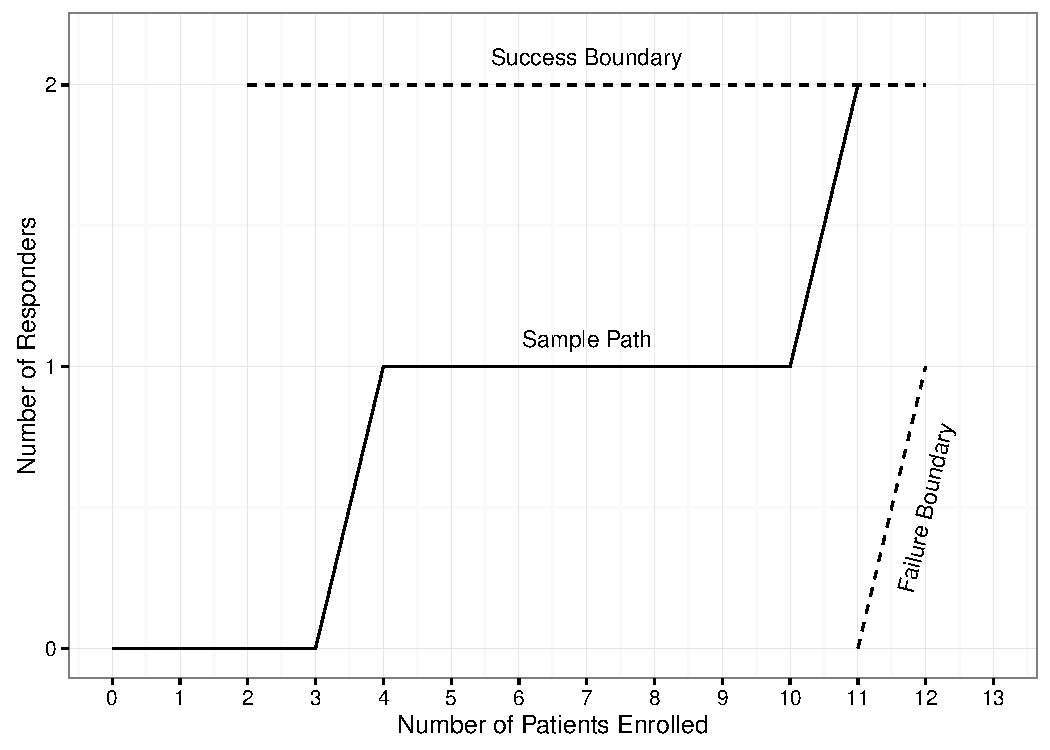
\includegraphics[width=\textwidth]{KanePlot.pdf}
\caption{
A hypothetical realization of the trial.
}
\label{fig:kane_viz}
\end{figure}

\begin{table}[t!]
\caption{Characteristics of the Stopped Negative Binomial Distribution}
\label{tab:snb}
\begin{center}
\begin{tabular}{|c|l|} \hline
Parameters & $p$ the success probability ($0\leq p \leq 1$; $q = 1-p$) \\
           & $s$ the number of successes before stopping ($s=1, 2, ...$)\\
           & $t$ the number of failures before stopping ($t=1, 2, ...$)\\ \hline
Support & min$(s,t) \leq k \leq s+t-1$  \\ \hline
$\mathbb{P}[Y=k]$ & ${k-1 \choose s-1} p^s (1-p)^{k-s} + {k-1 \choose t-1} (1-p)^s p^{k-t}$\\ \hline
$\mathbb{P}[Y \leq k]$ & $2 - \mathcal{I}_{q}(k+1, s) - \mathcal{I}_{p}(k+1, t)$\\ 
    & where $\mathcal{I}$ is the regularized incomplete beta function.\\ \hline
Mean & $\frac{s}{p} \mathcal{I}_p(s,t) + \frac{p^{s-1} q^{t-1}}{B(s,t)} +
  \frac{t}{q} \mathcal{I}_q(t,s) + \frac{p^{t-1} q^{s-1}}{B(s,t)}$\\ 
  & where $B$ is the beta function \\ \hline
MGF & $\left(\frac{p e^x}{1 - qe^x}\right)^s 
  \mathcal{I}_{1-qe^x} (s, t) + \left(\frac{qe^x}{1-pe^x}\right)^t 
  \mathcal{I}_{1-pe^x}(t, s) $\\ \hline
Compound Distribution & 
${k-1 \choose s-1} \frac{B\left(\alpha+s, k-s+\beta \right)}{B(\alpha, \beta)}+
{k-1 \choose t-1} \frac{B\left(\alpha + k-t, t+\beta\right)}{B(\alpha,\beta)}$\\
& for Beta($\alpha$, $\beta$). \\ \hline
\end{tabular}
\end{center}
\end{table}

In this work we derive the distribution of the number of enrollees needed
to observe either $s$ successes or $t$ failures. We refer to this distribution
as the Stopped Negative Binomial (SNB). Some of its characteristics are
summarized in Tab.~\ref{tab:snb}.
The rest of this paper derives these results
and explores properties of the distribution.
%The next section introduces our notation and basic results
%including the density of the distribution along with a description of
%its relation to other distributions. 
Section 2 derives the distribution function
based on a defined Bernoulli process and gives some basic properties.
Section 3 shows how the distribution is related to other standard
distributions and connects the SNB tail probability to the Binomial tail 
probability.
Section 4 derives the moment generating function.
Section 5 derives the compound distribution using a Beta distribution
for $p$. 

\section{Probability Mass Function}
\label{notation.section}

Let $\,b_1, b_2, \ldots \,$ denote a sequence of independent, identically
distributed, Bernoulli random variables with $\mathbb{P}[b_i=1]=p$ and
$\mathbb{P}[b_i = 0] = 1-p$, for
probability parameter $0\leq p \leq 1$. In the clinical trial setting
$\,b_i = 1$ corresponds to a successful patient outcome following treatment.  
Let $s$ and $t$ be positive integers.  Define the SNB random
variable $Y$ as the smallest
integer value such that $\,\{b_1, \ldots , b_Y\}\,$ contains {\em either}
$\,s\,$ successes {\em or} $\,t\,$ failures. That is, the SNB distribution
of $Y$ is the smallest integer such that either
$\sum_i^Y b_i = s$ or $\sum_i^Y 1-b_i = t$.

The distribution of $\,Y\,$ has support on integer values in the range
\begin{equation*}               
     \min(s,t) \leq \; Y \;\leq s+t-1  \label{range.y.eq}.
\end{equation*}
The probability mass function is
\begin{equation} \label{eqn:pmf}
\mathbb{P} [Y=k] = S(k, p, s) \ I_{\{s \leq k\}} + 
  S(k, 1-p, t) \ I_{\{ t \leq k \}}
\end{equation}
where $I_{\{f\}}$ is the {\emph indicator function}, taking the value 
of one if $f$ is true and zero otherwise, and
\begin{equation} \label{eqn:N}
S(k, p, s) = {k-1 \choose s-1} p^s (1-p)^{k-s} 
\end{equation}
is the negative binomial probability mass.

To prove (\ref{eqn:pmf}), consider the
process $\mathbf{X} = \left\{X(k) : k = 0,1,... \right\}$
with $X(0)=0$ and
\begin{equation*} \label{eqn:proc}
X_{k+1} = X_k + b_{k+1} \ I_{\{ k-t < X_k < s\}}.
\end{equation*}
At each step a patient's outcome is measured. In Fig.~\ref{fig:kane_viz} 
we consider a graphical illustration of the plot $X_k$ against
$k$. If the outcome of the $k$th patient is a success then the process 
advances diagonally in the positive horizontal and vertical direction. 
If the $k$th patient fails
then the sample path advances in the positive horizontal direction only. The
process continues until either $X_k = s$ or $X_k = k-t$.

\begin{prop}
The distribution of the stopping time
\begin{equation*}
Y = \argminl_k \left[X_k \geq s \cup X_k \leq k-t \right]
\end{equation*}
is given at (\ref{eqn:pmf}).
\end{prop}
\begin{proof}
%The proof will proceed in two parts. First, a combinatorial justification 
%will be given for the probability mass value on each element of the support. 
%Second, it will be shown that the sum of the masses over the support sums to 
%one.

The probability a given realization of $\mathbf{X}$ reaches $s$ at
the $k$th outcome is the probability that, at time $k-1$, there are $s-1$
successful outcomes and $k-s$ unsuccessful outcomes multiplied by
the probability of the final success at time $k$. This expression is given
in (\ref{eqn:N}). 
Similarly, the probability a given realization reaches $k-t$
is the probability that, at outcome $k-1$ there are $k-t$ successful outcomes
and $t-1$ unsuccessful outcomes multiplied by the probability of a final
unsuccessful outcome at time $k$.  

%Next, define
%\begin{equation} \label{stop_t}
%S'(k, p, t) = {k-1 \choose k-t} p^{k-t} (1-p)^t
%\end{equation}
%and notice that $S(k, p, s) = S'(k, 1-p, s)$ by writing
%\begin{equation*}
%{k-1 \choose k-s} = {k-1 \choose s-1}.
%\end{equation*}

To show that (\ref{eqn:pmf}) sums to one, define
%\begin{align} \label{eqn:sum_proof}
%R &= \sum_{k=s}^{s+t-1} S(k, p, s) + \sum_{k=t}^{s+t-1} S(k, 1-p, t) \\
%  &= \sum_{k=s}^{s+t-1} {k-1 \choose s-1} p^s (1-p)^{k-s} + \sum_{k=t}^{s+t-1} {k-1 \choose k-t} p^{k-t} (1-p)^t
%\end{align}
\begin{equation*} 
R = \sum_{k=s}^{s+t-1} S(k, p, s) + \sum_{k=t}^{s+t-1} S(k, 1-p, t).
\end{equation*}
If we substitute $i=k-s$ in the first summation and $j=k-t$ in the second then
$R$ can be written as the cumulative distribution function of two
negative binomial distributions:
\begin{equation} \label{eqn:transformed_sum}
R = \sum_{i=0}^{t-1} {i+s-1 \choose i} p^s (1-p)^i \; + \;
\sum_{j=0}^{s-1} {j+t-1 \choose j} p^j (1-p)^t.
\end{equation}

Let $\mathcal{I}_p(s, t)$ be the {\em regularized incomplete beta function} 
\citep{Olver2010}. This function satisfies 
$\mathcal{I}_p(s, t) = 1-\mathcal{I}_{1-p}(t, s)$ \citep{Uppuluri1970}. Then
\begin{align*}
R = \sum_{i=0}^{t-1} &{i+s-1 \choose i} p^s (1-p)^i +
\sum_{j=0}^{s-1}  {j+t-1 \choose j} p^j  (1-p)^t \\
   &= 1-\mathcal{I}_p(s, t) + 1 - \mathcal{I}_{1-p}(t, s) \\
   &= 1. 
\end{align*}
This completes the proof (\ref{eqn:pmf}) is the distribution of the
stopping time and is a valid probability mass function.
\end{proof}

Next, we consider an interim analysis of a clinical trial after $s'$ 
successes and $t'$ failures have been observed for $s' < s$ and $t' < t$.
\begin{corollary} \label{conditional_distribution}
The number of subsequent enrollments needed 
to reach either endpoint behaves as SNB($p$, $s-s'$, $t-t'$).
\end{corollary}
Having observed $s'$
successes and $t'$ failures, there are $s-s'$ successes needed to reach the
success endpoint and $t-t'$ failures needed to reach the failure endpoint.

\section{Connections and Approximations by Other Distributions}

\begin{figure}[p!]
\begin{center}
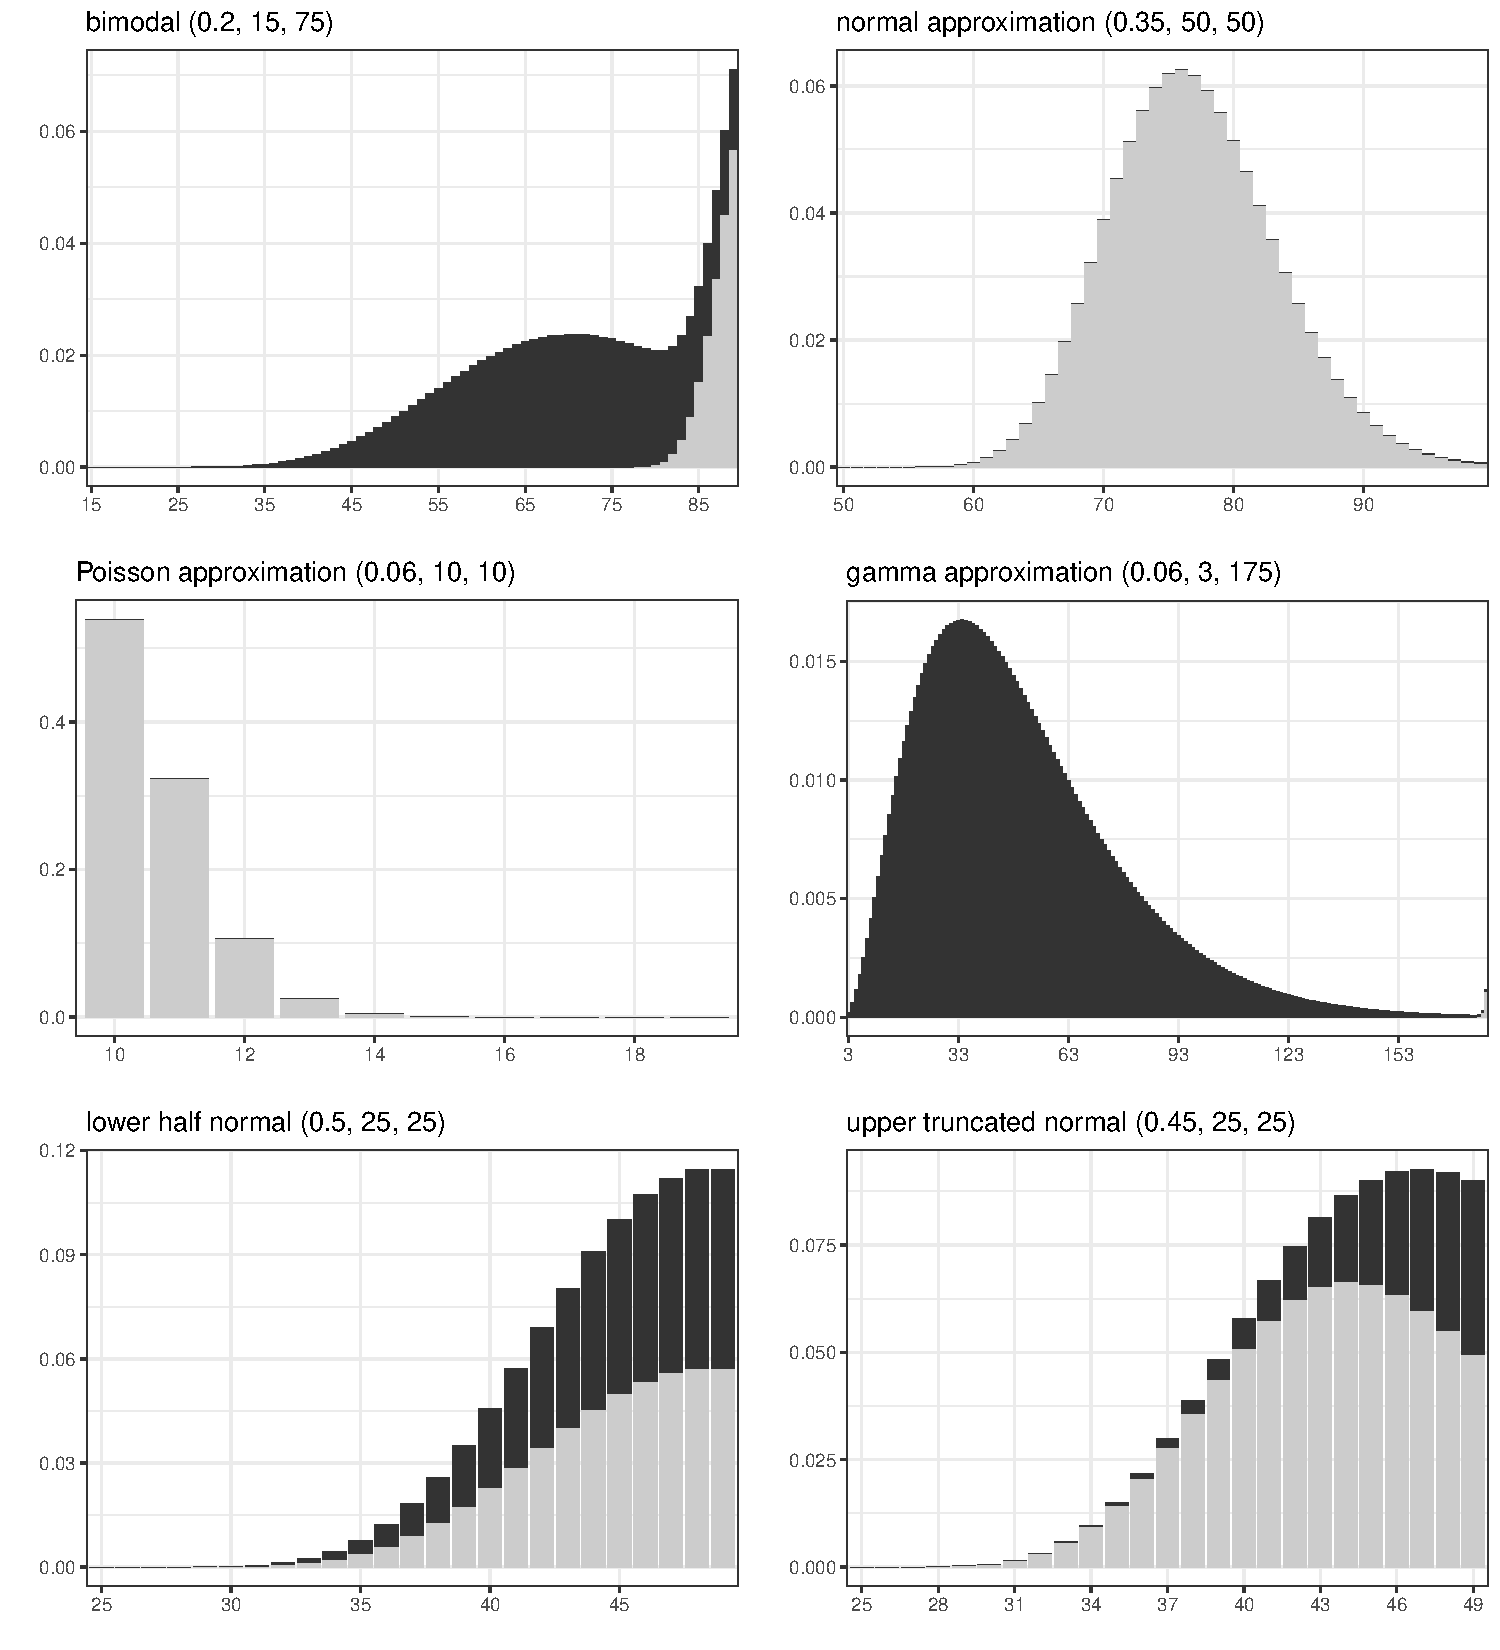
\includegraphics[width=\textwidth]{shapes.pdf}
\end{center}
\caption{Different shapes of the SNB distribution with parameters 
($p$, $s$, $t$), as given. Black indicates mass contributed by reaching
$s$ successes before $t$ failures. Grey indicates
mass contributed by reaching $t$ failures first. \label{shapes.fig}}
\end{figure}

The SNB is a generalization of the negative 
binomial distribution. If $t$ is large then $Y-s$ has a 
negative binomial distribution with
\begin{equation*}                                    %   (1)   
\mathbb{P}[Y=s+j]        \label{nb1.eq}          
  = {{s+j-1}\choose{s-1}} p^s (1-p)^j
\end{equation*}
for $\,j=0, 1,\ldots\,$. A similar statement can be made when $s$ is large
and $t$ is small. As a result, with proper parameter choice, the SNB
can mimic other probability distributions in a manner similar to 
those described in \cite{Peizer1968} and \cite{Best1974}. Examples are
shown in in Fig.~\ref{shapes.fig}. 

The SNB also generalizes both the minimum (riff-shuffle) and maximum negative
binomial distributions up to a translation of the support.
For the special case of $\,s=t,$ the distribution of $\,Y\,$ is the
riff-shuffle, or minimum negative binomial distribution~\citep{Uppuluri1970}.
Similar derivations of the closely-related maximum negative binomial 
discrete distributions also appear in~\cite{Zhang2000}
and \cite{Zelterman2005}.
The maximum negative binomial is the smallest number of outcomes necessary to 
observe at least $s$ successes {\em and} $s$ failures. The SNB is the 
number of outcomes to observe {\em either} $s$ successes or $t$ failures.

%\section{Connection Between the SNB and the Binomial Tail Probability}

There is a close connection between the tail probabilities of the SNB and the 
binomial distributions.
The probability of reaching the success endpoint in an 
SNB($p$, $s$, $t$) random variable is 
equal to the probability of at least $s$ successes in a Binomial distributed 
random variable with size $s+t-1$ and success probability $p$. 
Likewise, the probability of reaching the failure endpoint is equal
to the probability of at most $s-1$ successes in a Binomial distribution. 
That is, the probability that the number of successes is at least $s$ in the 
Binomial model is the same that the treatment succeeds (reaches $s$) in the SNB 
model.
\begin{prop} \label{binomial_tail}
Let $Y$ be distributed as SNB($p$, $s$, $t$) and let 
$B$ be distributed Binomial with size $n=s+t-1$ and success probability
$p$. Then
\begin{equation}
\mathbb{P}[B \geq s] = \mathbb{P} [\text{treatment succeeds}].
\end{equation}
\end{prop}
\begin{proof}
The Binomial tail probability is
\begin{equation*}
\mathbb{P}[B \geq s] = 1 - \mathcal{I}_{1-p}.
\end{equation*}
%\begin{align*}
%\mathbb{P}[B \geq s] &= \sum_{k=s}^{s+t-1} {n \choose k} p^k (1-p)^{n-k} \\
%  &= 1 - \sum_{k=0}^{s-1} {n \choose k} p^k (1-p)^{n-k} \\
%  &= 1 - \mathcal{I}_{1-p}.
%\end{align*}
The corresponding SNB probability is
\begin{equation*}
\mathbb{P} [\text{treatment succeeds}] 
  = \sum_{k=s}^{s+t-1} {k-1 \choose s-1} p^s (1-p)^{k-s}.
\end{equation*}
Let $i=k-s$. Using the fact that
\begin{equation*}
{i+s-1 \choose s-1} = {i+s-1 \choose i}
\end{equation*}
the last summation can be rewritten as
\begin{align}
\mathbb{P} [\text{treatment succeeds}] &= \sum_{i=0}^{t-1} 
  {i+s-1 \choose i} p^s (1-p)^i\\
  &= 1 - \mathcal{I}_{1-p}(t, s)
\end{align}
completing the proof.
\end{proof}

To illustrate this result, let us return to our initial example
where $s=2$, $t=12$, and $p=0.045$.  The probability masses in
Fig.~\ref{fig:snb_bin_compare} represented in 
black are equal in panels a) and b) as are the masses in grey.
The probability that $s$
successes are reached in the SNB process is the same as the binomial 
probability of at least two successes. Likewise, the probability that $t$ 
failures are reached in the SNB process is the same as the binomial
probability of zero or one successes.

\begin{figure}[t!]
\centering
\subfloat[The SNB distribution.]{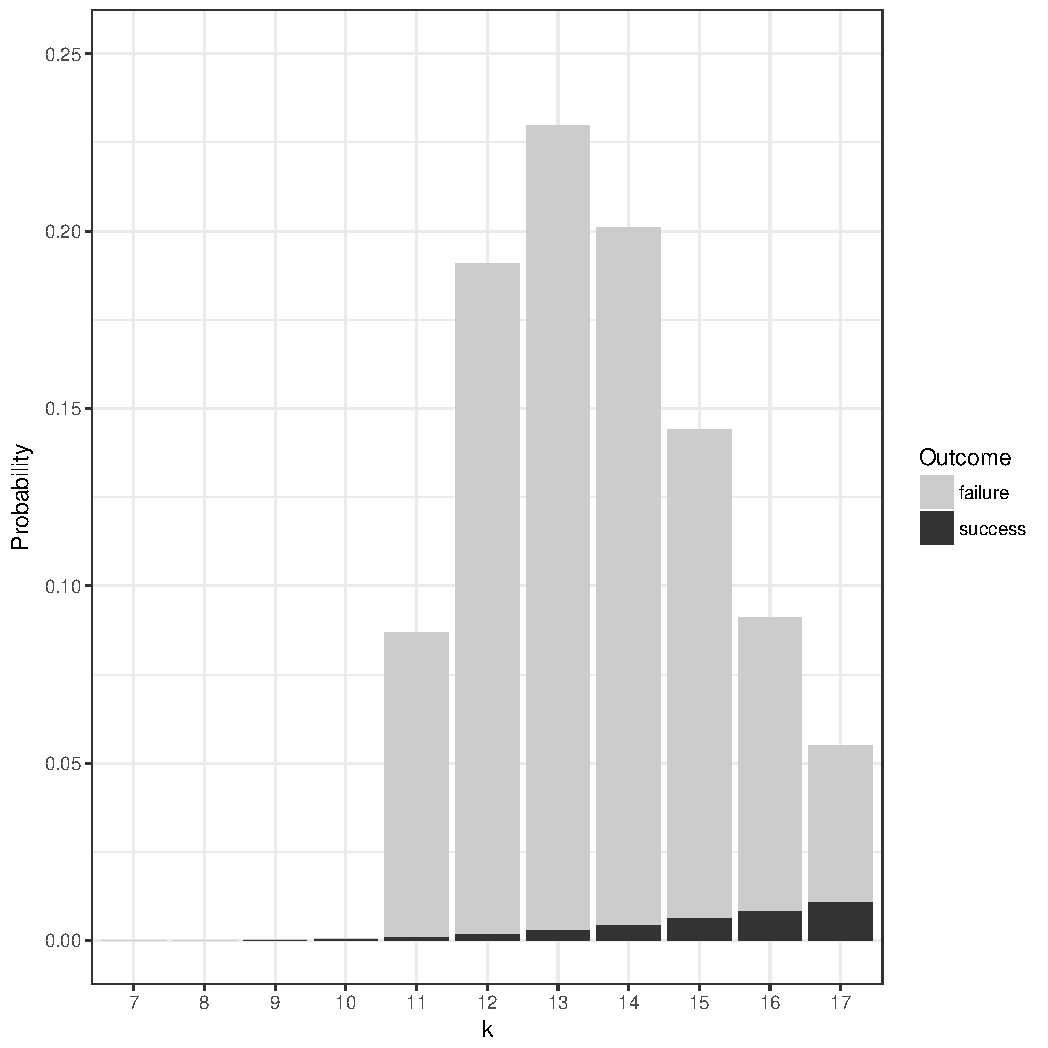
\includegraphics[width=0.5\textwidth]{snb_density.pdf}}
\hfill
\subfloat[The Binomial distribution.]{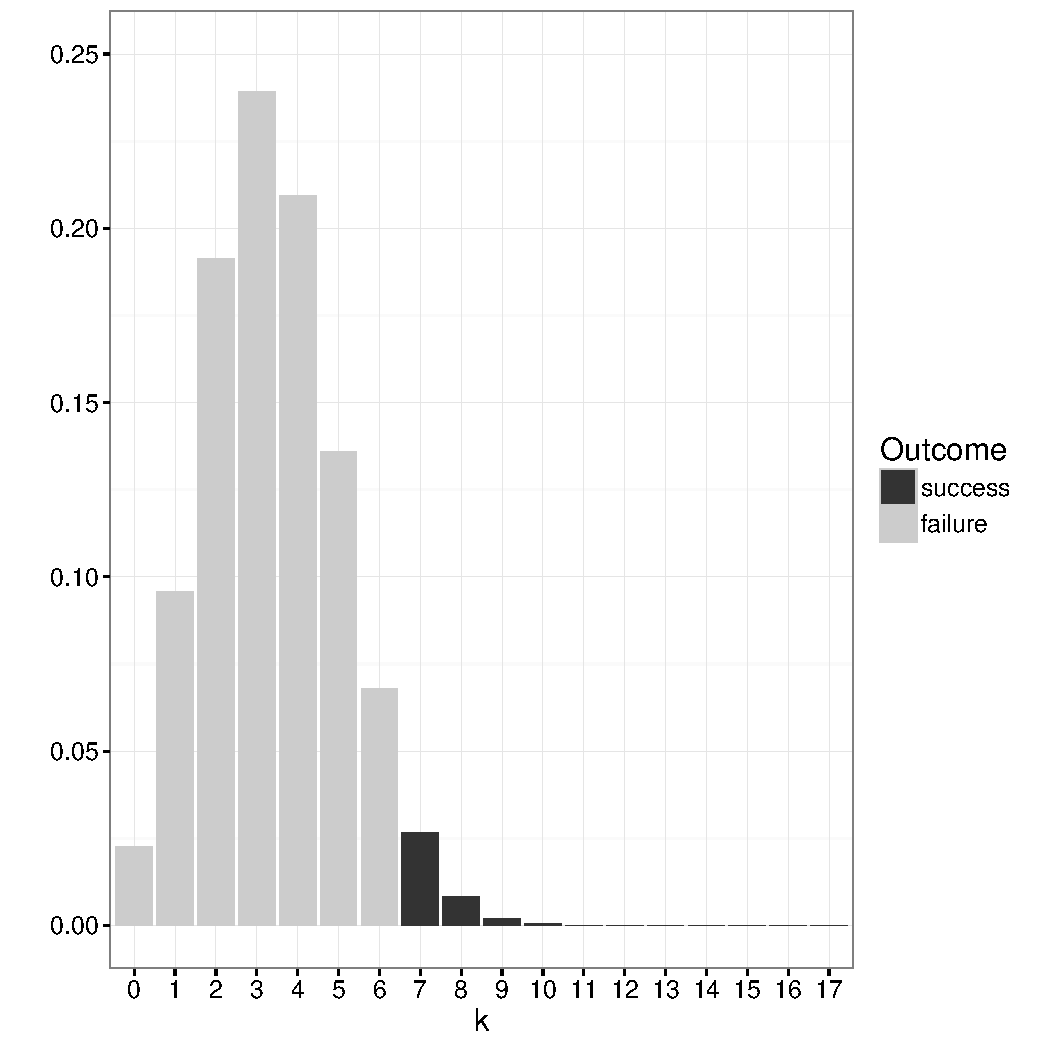
\includegraphics[width=0.5\textwidth]{bin_density.pdf}}
\caption{
SNB(0.045, 2, 12) with mass contributed from 
$s$ successes (black) or $t$ failures (grey) along with Bin(0.045, 12) with
at least 2 successes (black) or fewer (grey).
}
\label{fig:snb_bin_compare}
\end{figure}

\section{The Moment Generating Function}

The moment generating function for the SNB is calculated in a manner similar to 
that of two negative binomial distributions. 
\begin{prop} Let $Y$ be distributed SNB with parameters $p$, $s$, and $t$.
Then the moment generating function (MGF) of $Y$ is
\begin{equation} \label{eqn:mgf}
\mathbb{E}~e^{xY} = \left(\frac{p e^x}{1 - qe^x}\right)^s 
  \mathcal{I}_{1-qe^x} (s, t) + \left(\frac{qe^x}{1-pe^x}\right)^t 
  \mathcal{I}_{1-pe^x}(t, s)
\end{equation}
for $q = 1-p$ when $x \leq \min \left\{\log(1/p), \log(1/q) \right\}$.
\end{prop}
\begin{proof}
The MGF of the SNB is:
\begin{equation*}
\mathbb{E}~e^{xY} = \sum_{k=s}^{s+t-1} {k-1 \choose s-1} p^s q^{k-s} e^{kx} 
  + \sum_{k=t}^{s+t-1} {k-1 \choose t-1} p^{k-t} q^t e^{kx}
\end{equation*}
and can be rewritten as:
\begin{equation} \label{eqn:first_sum}
\mathbb{E}~e^{xY} = \sum_{k=s}^{s+t-1}{k-1 \choose s-1} (pe)^{sx} (qe^x)^{k-s} 
  + \sum_{k=t}^{s+t-1}{k-1 \choose t-1} (qe^x)^t (pe^x)^{k-t}.
\end{equation}
The first summation in (\ref{eqn:first_sum}) satisfies
\begin{align*}
\sum_{k=s}^{s+t-1}{k-1 \choose s-1} (pe)^{sx} (qe^x)^{k-s} &= 
  \left(\frac{pe^x}{1 - qe^x}\right)^s \ \ \sum_{k=s}^{s+t-1} {k-1 \choose s-1} 
    (qe^x)^{k-s} (1-qe^x)^s \\
  &= \left(\frac{pe^x}{1 - qe^x}\right)^s \mathcal{I}_{qe^x}(s, t).
\end{align*}
Since the incomplete beta function's subscript parameter has support on zero 
to one, we have $qe^x \leq 1$. This also shows we must restrict
$x \leq -\log(q)$.
A similar expression can be derived for the second summation in 
Equation \ref{eqn:first_sum} and results in
the constraint $x \leq -\log(p)$.
\end{proof}

The SNB's ability to approximate the geometric, normal, and gamma 
distributions follow from it generalizing the negative binomial. To 
recover the MGF of the negative binomial consider the case where
$t \rightarrow \infty$ in (\ref{eqn:mgf}). The regularized incomplete
beta function in the first term goes to one and zero in the second term
and we are left with the MGF of the negative binomial distribution. 
When $s=1$ this is the same as the geometric distribution. The negative
binomial can therefore be seen as a sum of i.i.d. geometric distributions.
For an appropriately large number of samples the central limit theorem
hold yielding a normal approximation.

Drawing a connection to the gamma distribution is more complicated.
However it is a well-studied problem in the literature (see 
\cite{Ord1968,Guenther1972,Best1974} for examples). Methods for these
approximation generally work by equating cumulants and then showing 
that errors are not too far off. 

The lower-half normal distribution can be approximated by setting $s=t$
for appropriately large $s$ and $t$ and $p = 0.5$. In this
case the SNB can be viewed as identical, negative binomials
approximating a normal and truncated at the median.

\section{The Compound Probability Distribution}

Let us consider a Bayesian analysis with a Beta distribution on $p$.
\begin{prop} \label{prop:bayesian}
The compound distribution of the Stopped Negative Binomial 
distribution when $p$ is distributed Beta($\alpha$, $\beta$) is
\begin{align} \label{eqn:posterior}
\mathbb{P} [Y = k | s, t, \alpha, \beta ] &= 
  {k-1 \choose s-1} \frac{B\left(\alpha+s, k-s+\beta \right)}{B(\alpha, \beta)} 
    \ I_{\{s \leq k \leq s+k-1\}} \ + \nonumber \\
  & {k-1 \choose t-1} 
    \frac{B\left(\alpha + k - t, t+\beta\right)}{B(\alpha, \beta)} 
    \ I_{\{t \leq k \leq s+k-1\}}.
\end{align}
\end{prop}
\begin{proof}
For notational simplicity, assume that $k$ is in the range
$\min(s,t) \leq k \leq s+t-1$. When 
this is not the case appropriate terms should be removed as dictated by the indicator functions.
\begin{align*}
f(k | s, t, \alpha, \beta) = \frac{1}{B(\alpha, \beta)} & \int_0^1 {k-1 \choose s-1} p^{\alpha +s -1} \left(1-p\right)^{k-s+\beta-1} + \\
 & {k-1 \choose t-1} p^{k-t+\alpha-1}\left(1-p\right)^{t+\beta-1} dp \\
= \frac{1}{B(\alpha, \beta)}  {k-1 \choose s-1} & \int_0^1  p^{\alpha +s -1} \left(1-p\right)^{k-s+\beta-1} dp + \\
 & \frac{1}{B(\alpha, \beta)} {k-1 \choose t-1} \int_0^1  p^{k-t+\alpha-1}\left(1-p\right)^{t+\beta-1} dp.
\end{align*}
The result in (\ref{eqn:posterior}) follows by the definition of the 
Beta function.
\end{proof}

To better understand the compound distribution, let us once again return to 
our example where $s=2$, $t=12$. However, we assume $p$ is a Beta distribution
with shape parameters $\alpha = 0.045 c$ and 
$\beta = 0.955 c$ for any $c > 0$.
This parameterization allows us to examine the relationship between 
uncertainty in $p$ and the SNB.

\begin{figure}[t!]
\centering
\subfloat[The compound distribution's expected sample size.]{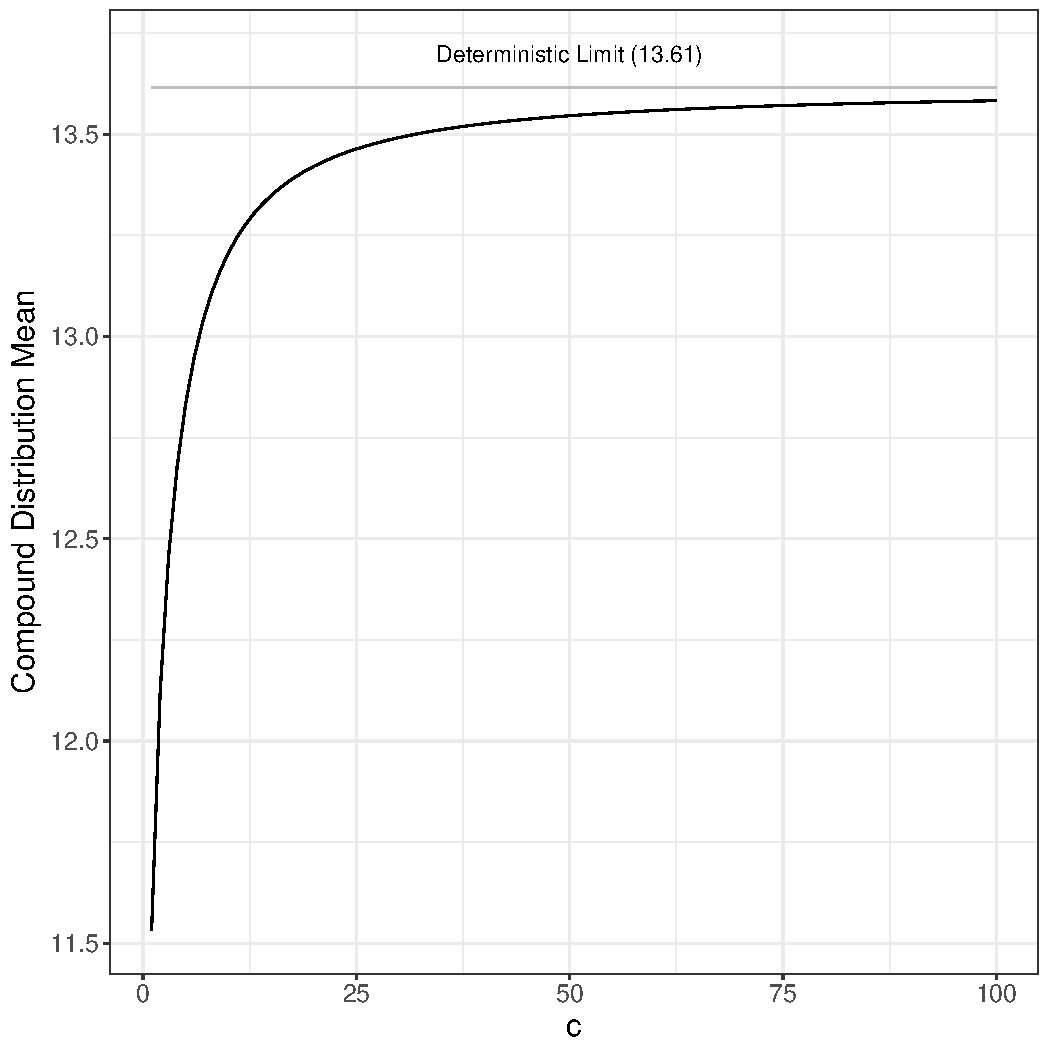
\includegraphics[width=0.5\textwidth]{bayesian-sample-expectation.pdf}}
\hfill
\subfloat[The compound distribution's variance.]{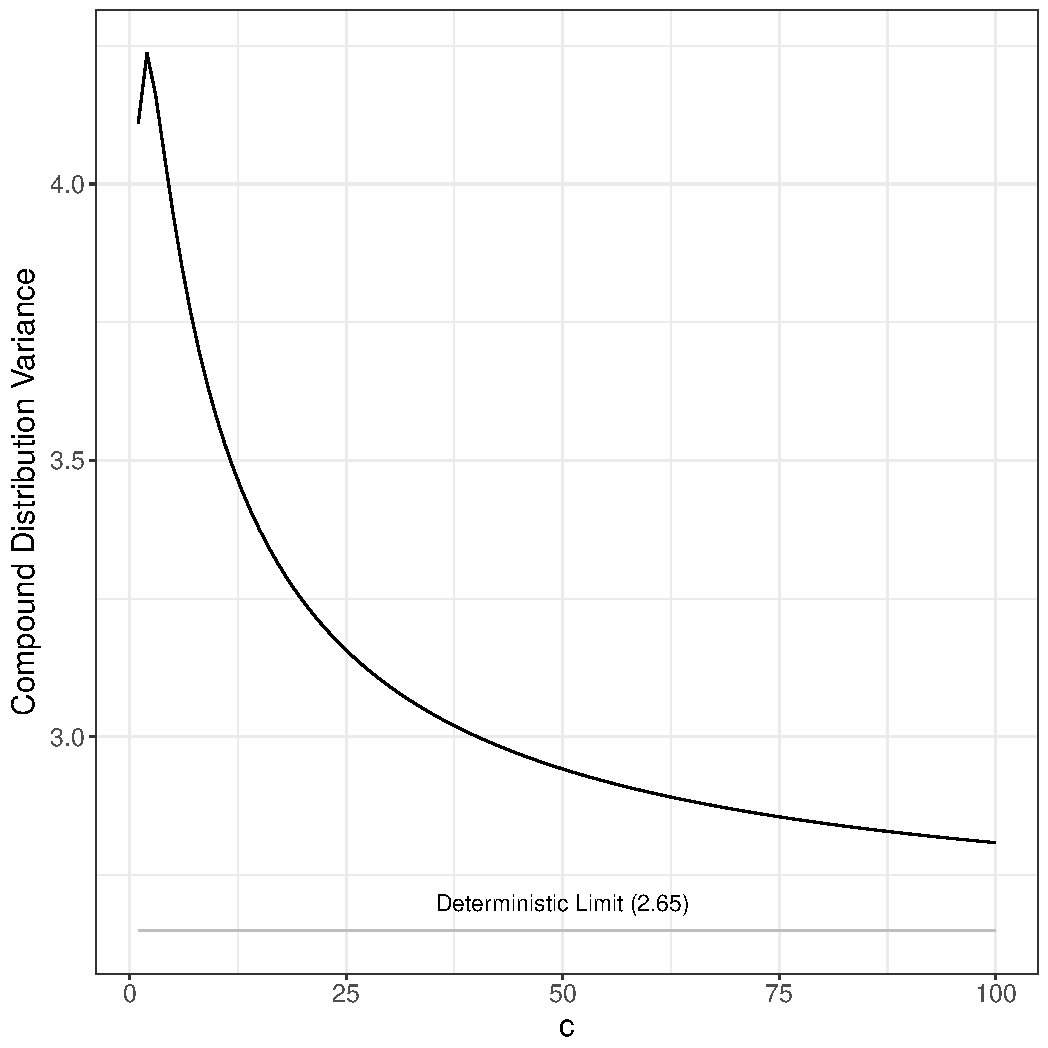
\includegraphics[width=0.5\textwidth]{bayesian-sample-variance.pdf}}
\caption{
The expected size and variance of the compound SNB with $s=2$, $t=12$
with $\mathbb{E}\ p = 0.045$ varying the uncertainty 
in the distribution of $p$. A larger value of $c$
corresponds to a Beta with smaller variance.
}
\label{fig:bayesian-sample-size}
\end{figure}

Fig.~\ref{fig:bayesian-sample-size} shows how the expected sample size
and variance of the compound SNB. As the certainty increases the 
compound distribution sample values converge to corresponding expected 
values with 
$p = 0.045$. It may be noted that the compound distribution's mean
approaches the deterministic limit slowly. This
is because when $c$ is small, the distribution of $p$ is heavily skewed. 
As $c$ increases this effect is minimized.

Slow convergence in the mean will occur when $p$ takes values close to 
zero or one. In these cases it may be preferable to select shape parameters
based on the median or mode of the beta distribution. These values
will vary less in the uncertainty of the distribution.

%\section{Discussion}
%
%The SNB can be used to extend clinical trial methodology
%in at least two areas. First, it can be used to construct nested criteria
%for early stopping and efficacy. Current approaches are often inspired by
%the Simon 2-stage Phase II clinical trial \cite{Simon1989} where a
%a small number of patients are enrolled for an initial stage. For patients,
%success or failure is assessed. If at least a pre-specified number of
%successes are observed then the trial enters a second stage with more
%patients. If a sufficient number of successes are not observed then the
%trial fails. 

%The SNB is being used to generalize the Simon design by providing separate
%criteria for futility and efficacy.
%The Simon design tests for a single response probability and time-to-event
%parameter for both the first
%and second stage. The SNB is being used to generalize this design by 
%allowing these parameters to vary for the two stages, and even allow
%information about patients in the first stage to be used in the second
%stage. Early results show the design provides
%both early testing for futility along with the ability
%to make statistically sound decisions sooner than traditional trials.

%A second avenue for methodological innovation comes directly from
%Corollary \ref{conditional_distribution} and Proposition \ref{prop:bayesian}.
%Our knowledge of the response probability $p$ comes from published reports
%yielding a prior distribution.
%While a trial is being conducted the response probabilities are 
%updated as new results are received. The number of individual successes
%and failure are used to learn the shape characteristics of the corresponding
%Beta distribution and resulting posterior
%distribution. An estimate of the probability of reaching the success (and
%failure) endpoints can be provided at each step of the trial.

%There are also several avenues for extending the SNB itself. First is the 
%development of a stopped negative multinomial distribution allowing
%for more than two endpoints. This extension would have clinical trial
%applications including dose escalation where the outcomes are response
%to a therapy, failure to respond, and an adverse outcome endpoint where
%an enrollee is removed from the trial with neither response or non-response
%due to side effects.

%A second, more theoretical extension is to the asymptotic setting. Under
%proper reparameterization, the process from which the SNB is derived 
%can be shown to converge to a Brownian motion. In this case, we conjecture
%that the SNB can be defined in terms of the L\'{e}vy-Bachelier 
%\citep{Bachelier1900} formula
%thereby relating the SNB to the classic result in stochastic calculus.

\section*{References}

\bibliography{mybibfile}

\end{document}
